\documentclass[12pt,portuguese]{beamer}
\usepackage[T1]{fontenc}
\usepackage[utf8]{inputenc}
\usepackage[brazil]{babel}

\mode<presentation>
{
	\usetheme{Boadilla}
%  \usetheme{Madrid}       % or try default, Darmstadt, Warsaw, ...
%  \usecolortheme{default} % or try albatross, beaver, crane, ...
%  \usefonttheme{serif}    % or try default, structurebold, ...
%  \setbeamertemplate{navigation symbols}{}
%  \setbeamertemplate{caption}[numbered]
} 
\usepackage[round]{natbib}
\usepackage{caption}
\usepackage{algorithm}
\usepackage[noend]{algpseudocode}
\usepackage{comment}
\usepackage{amsmath}

\setbeamertemplate{bibliography entry title}{}
\setbeamertemplate{bibliography entry location}{}
\setbeamertemplate{bibliography entry note}{}

\title{An Evolutionary Approach for Forex Trading Based on Technical Indicators}
%\author{Victor Hugo Cândido de Oliveira}
%\institute{ICMC/USP}
\author[Delbem, A. C. B.]{Alexandre C. B. Delbem \inst{1} \\
	\and Geraldo Silva \inst{2} \\
	\and Victor Hugo Cândido de Oliveira \inst{1}}
\institute[ICMC/USP]{\inst{1} ICMC/USP \and %
                      \inst{2} IBILCE/UNESP}
\date{01 de Dezembro de 2016}

\begin{document}


%\AtBeginSection[]
%{
%	\begin{frame}{Outline}
%	\tableofcontents[currentsection,subsectionstyle=hide,subsubsectionstyle=hide]
%	\end{frame}
%}

%\AtBeginSubsection[
%	{\frame<beamer>{\frametitle{Outline}   
%	\tableofcontents[currentsubsection]}}%
%]%
%{
%  \frame<beamer>{ 
%    \frametitle{Outline}   
%    \tableofcontents[currentsubsection]}
%}
\AtBeginSubsection[]{
\begin{frame}<beamer>
	\frametitle{Outline}
%\tableofcontents[currentsection,sectionstyle=hide/hide/hide/show/hide,currentsubsection=hide/hide/hide/show/hide,subsubsectionstyle=hide]
	\tableofcontents[
	currentsection,
	sectionstyle=show/show,
	subsectionstyle=show/shaded/hide]
\end{frame}
}


\maketitle

\section{Technical Analysis}
\subsection{Definition}
\begin{frame}{Definition}
\begin{itemize}
	\item \citet{Murphy1999} defines Technical Analysis as ``the study of market action, primarily through the use of charts, for the purpose of forecasting future price trends''

		\pause
	\item Market action information sources \citep{Murphy1999}:
	\begin{itemize}
		\item Price
		\item Volume
		\item Open interest
	\end{itemize}

		\pause
	\item Philosophy \citep{Murphy1999}:
	\begin{itemize}
		\item Market action discounts everything
		\item Prices move in trends
		\item History repeats itself
	\end{itemize}
\end{itemize}
\end{frame}

\subsection{Technical Indicators}
\begin{frame}{Simple Moving Average -- SMA}
	$$SMA(p,n) = \sum_{i=1}^n \frac{p_i}{n}$$

	Examples of SMA\footnote{\url{http://www.fmlabs.com/reference/default.htm?url=SMA.htm}} with 5, 30 and 80 periods:
	\begin{figure}[H]
	\centering
	%\includegraphics[page=4,width=0.8\textwidth]{images/chart_SMA_AUDCAD.pdf}
	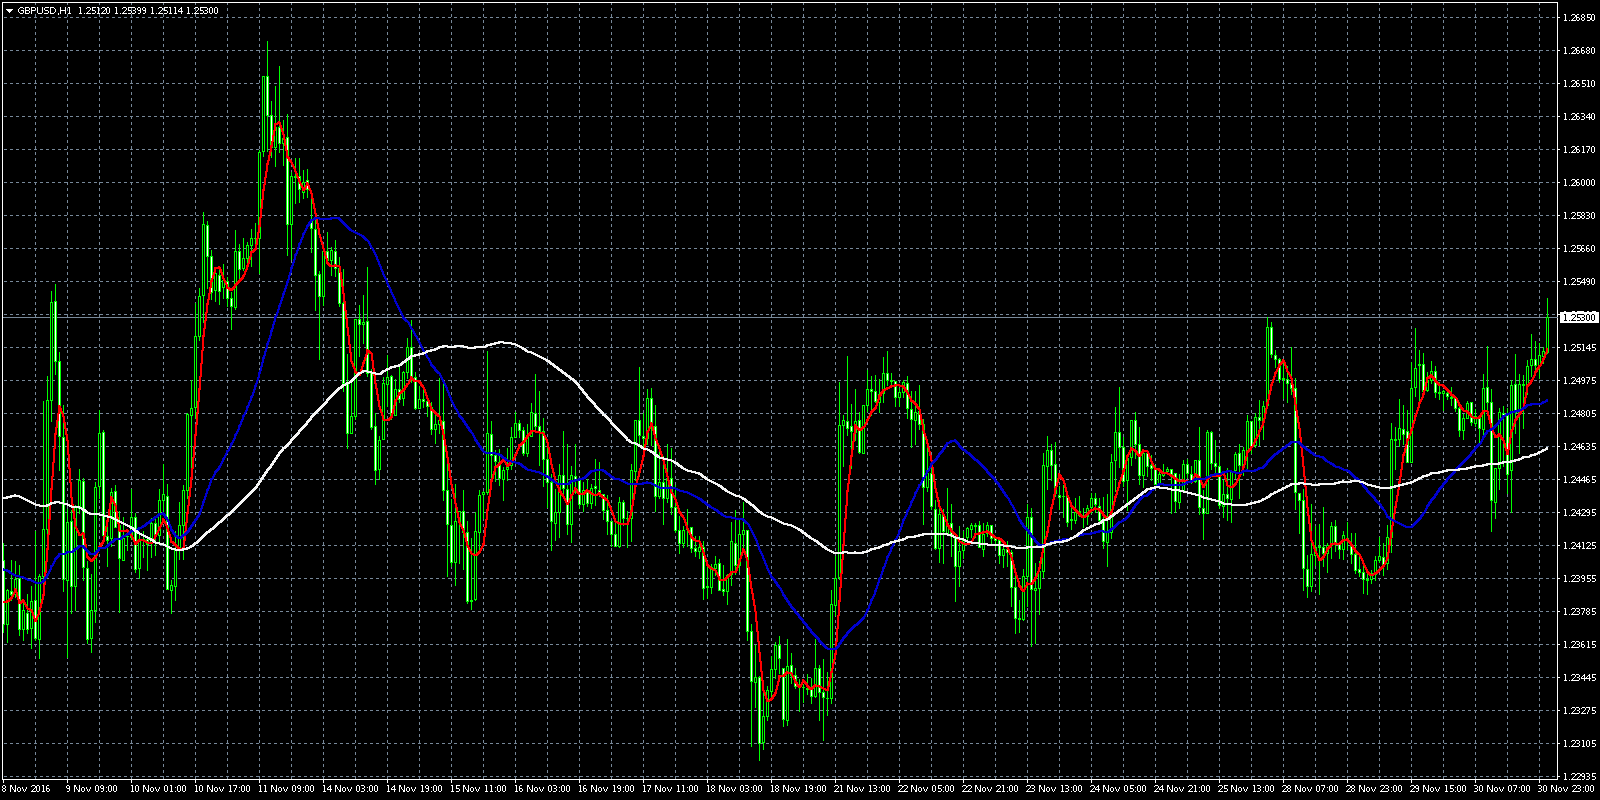
\includegraphics[width=0.8\textwidth]{images/mt4_SMA.png}
	\end{figure}
\end{frame}

\begin{frame}{Relative Strength Index -- RSI}
\begin{equation*}
\begin{array}{rcl}
RSI(p,n) & = & 100 - \frac{100}{1-RS}
\\
RS & = & \frac{AvgUp}{AvgDn}
\end{array}
\end{equation*}

	Example of RSI \citep{WilderJr1978} with 14 periods:
	\begin{figure}[H]
	\centering
	%\includegraphics[page=2,width=0.8\textwidth]{images/chart_RSI_AUDCAD.pdf}
	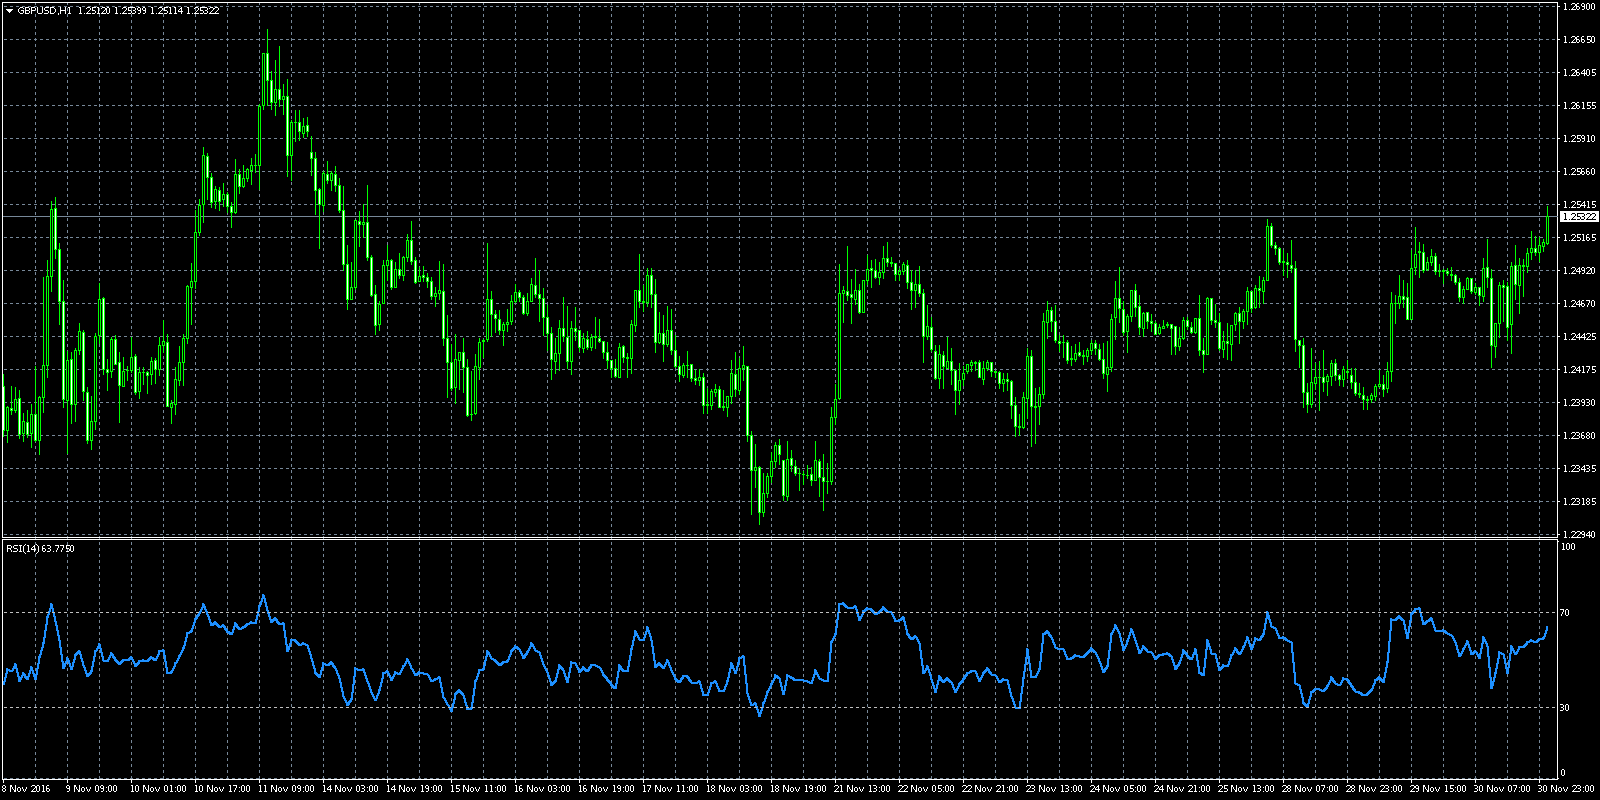
\includegraphics[width=0.8\textwidth]{images/mt4_RSI.png}
	\end{figure}
\end{frame}

\begin{frame}{Stochastic Oscilator}
\begin{equation*}
\begin{array}{rcl}
	\%K &=& \frac{close - lowest(n_K)}{highest(n_K) - lowest(n_K)}
\\
	\%D & = & MA(\%K, n_D)
\end{array}
\end{equation*}

	Example of Stochastic Oscilator \citep{Lane1984} with $n_K=14, n_D=3$ periods:
	\begin{figure}[H]
	\centering
	%\includegraphics[page=2,width=0.8\textwidth]{images/chart_stoch_AUDCAD.pdf}
	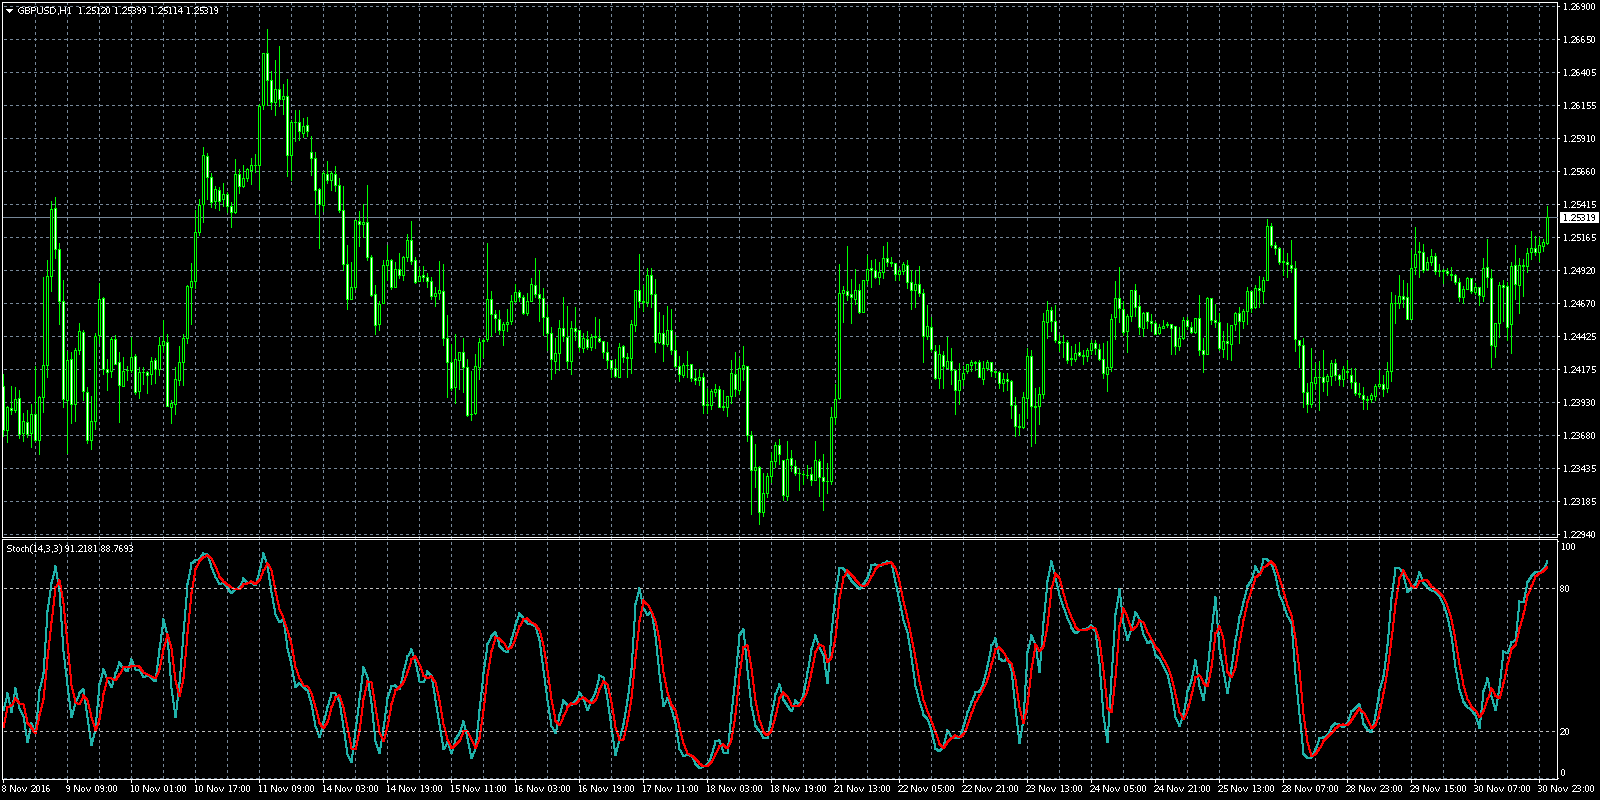
\includegraphics[width=0.8\textwidth]{images/mt4_stoch.png}
	\end{figure}
\end{frame}

\begin{frame}{Stochastic RSI}
	Apply Lane's Stochastic Oscilator over Wilder's Relative Strength Index

	\begin{figure}[H]
	\centering
	%\includegraphics[page=2,width=0.8\textwidth]{images/chart_stoch_AUDCAD.pdf}
	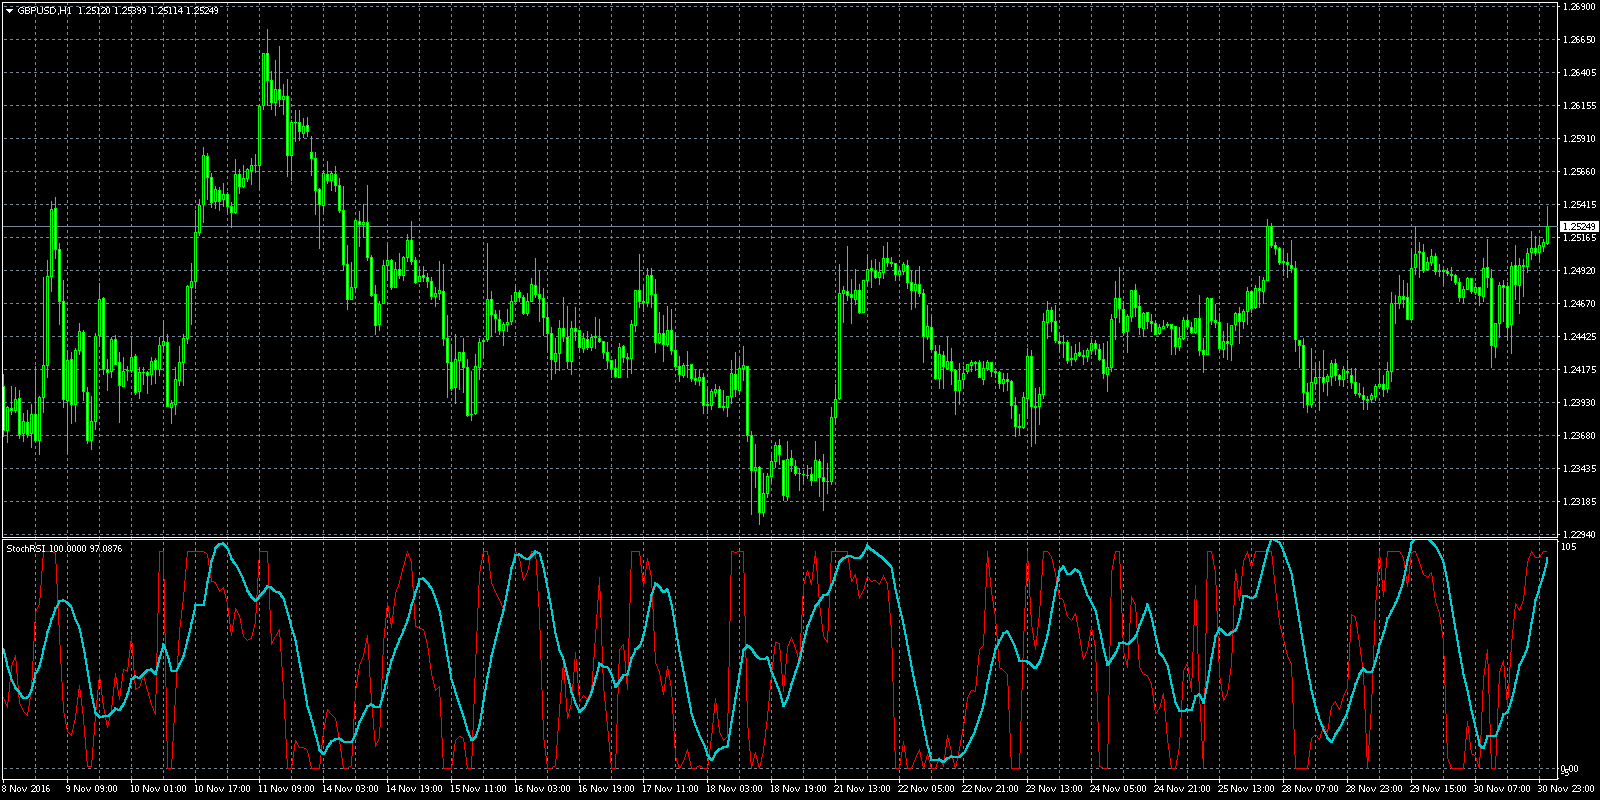
\includegraphics[width=\textwidth]{images/mt4_stochRSI.png}
	\end{figure}
\end{frame}

\begin{frame}{Fibonacci Retracement Lines}
	Fibonacci Retracement Lines are placed according to some ratios present in the Fibonacci sequence\footnote{\url{http://stockcharts.com/school/doku.php?id=chart_school:chart_analysis:fibonacci_retracemen}}:
\begin{equation*}
\begin{array}{rcl}
	F_{n+1} = F_n + F_{n-1}\\
	\\
	\frac{F_n}{F_{n-1}} \approx 1.618 \\
	\\
	\frac{F_n}{F_{n+1}} \approx 0.618 \\
	\\
	\frac{F_n}{F_{n+2}} \approx 0.382 \\
	\\
	\frac{F_n}{F_{n+3}} \approx 0.236 \\
\end{array}
\end{equation*}
\end{frame}
	
\begin{frame}{Fibonacci Retracement Lines}
	These lines are used as support and resistance levels
	\begin{figure}[h]
	\centering
	%\includegraphics[page=2,width=0.8\textwidth]{images/chart_stoch_audcad.pdf}
	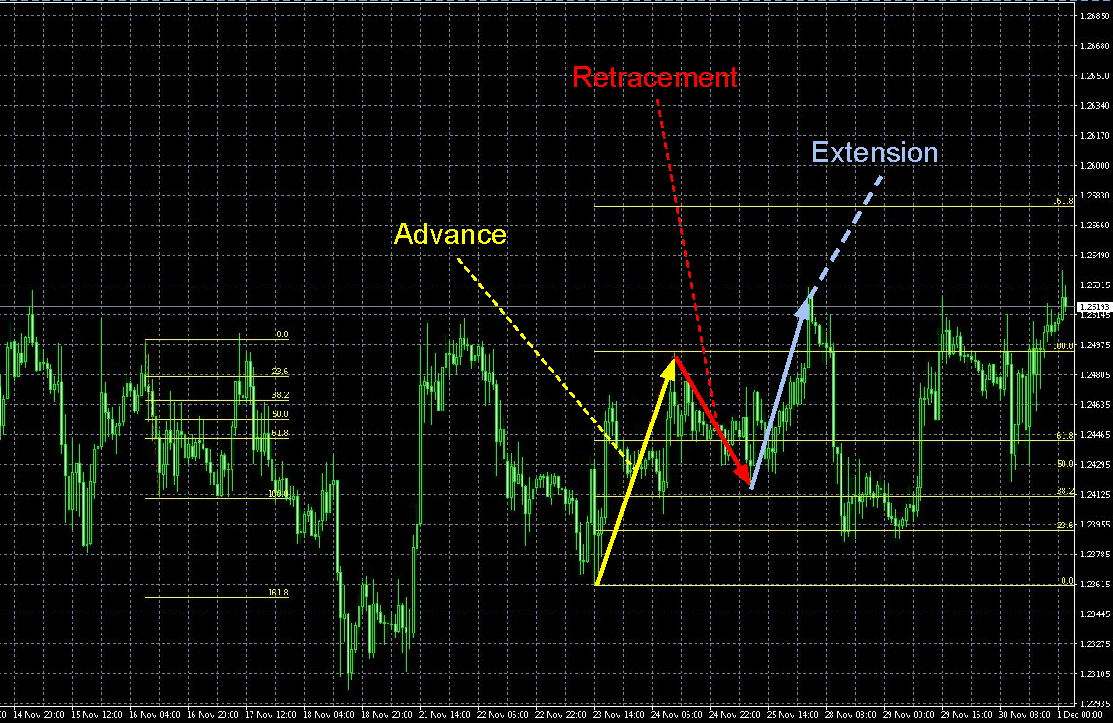
\includegraphics[width=0.9\textwidth]{images/mt4_fibo.pdf}
	\end{figure}
\end{frame}

\section{Currency Strength Strategy}
\subsection{Currencies}
\begin{frame}{Currency Strength Strategy}
	Based on the strength of the following currencies and the 21 currency pairs resulting of their combination

\begin{table}[!htb]
	\centering
	\begin{tabular}{c|c}
		Symbol & Name \\ \hline\hline
		AUD & Australian Dollar \\
		CAD & Canadian Dollar \\
		EUR & Euro\\
		GBP & Pound Sterling \\
		JPY & Japanese Yen \\
		NZD & New Zealand Dollar \\
		USD & United States Dollar \\
	\end{tabular}
\end{table}

	%\vspace{3pt}
	%Available at: \url{https://github.com/vhcandido/currency-strength}
\end{frame}

\subsection{Strength Matrixes}
\begin{frame}{Currency Strength -- Strength Matrixes}
\begin{itemize}
	\item Matrix 1: if the current price is above $SMA(Close, n)$ \\ $\rightarrow m \in \{-1,1\}$
	\item Matrix 2: if the current price has retracted to Fibonacci's 0.382 level (using $SMA(Close, n)$)\\ $\rightarrow m \in \{-1,0,1\}$
	\item Matrix 3: $M1 + M2 \rightarrow m \in [-2,2] \cap \mathbb{Z}$
	\item Vector 4: sum of columns for each line $\rightarrow v \in [-12,12] \cap \mathbb{Z}$
		$$v[i] = \sum_{j=1}^7 x_{ij}, i=1,2, ..., 7$$
	\item Matrix 4: strength difference between currencies $\rightarrow m \in [-24,24] \cap \mathbb{Z}$
\end{itemize}
\end{frame}

\subsection{Selecting Currencies}
\begin{frame}{Currency Strength -- Selecting Currencies}
	Loop in time, taking risk per order and maximum risk into account.
\begin{itemize}
	\item Choose, based on $M4$, the group of pairs with the higher strength difference ($>= 6$)
	\item Do not choose pairs which currencies have absolute strength (vector 4) below 4
	\item Some definitions
		\begin{itemize}
			\item Stop loss is placed 15 pips below the last bottom
			\item Take profit is placed $3*(current-SL)$ pips above current price (TP:SL = 3:1)
			\item Stochastic RSI: $stoch(RSI(n=14), fastK=5, fastD=5, slowD=3)$, using $fastD$ ($\%D$)
		\end{itemize}
\end{itemize}
\end{frame}

\subsection{Order Management}
\begin{frame}{Estratégia de Julho -- Order Management}
\begin{itemize}
	\item Order is open following the strength given by Matrix 4. BUY order example:
		\begin{itemize}
			\item Current price is above $SMA(High, n)$ by at least 5 pips
			\item Stochastic RSI is below 20\% or 70\% but falling
			\item Pair strength given by $M3$ is 2 (max)
			\item Last bottom must be below current price
			\item When the candle opens below last top price the SL is updated to 15 pips below the last bottom
		\end{itemize}
	\item Lot size is calculated based on risk per order
\end{itemize}
\end{frame}

\section{Evolutionary Approach}
\subsection{Genetic Algorithms}
\begin{frame}{Genetic Algorithms}
\begin{itemize}
	\item Developed by \citet{Holland1975}, Genetic Algorithms are probabilistic search methods inspired by natural selection and genetics \citep{Gaspar2012}.
	\item Reproduction, competition, mutation and selection
\end{itemize}
\begin{center}
\scalebox{0.65}{
\begin{minipage}{1.3\linewidth}

\begin{algorithm}[H]
	\caption{Genetic Algorithm Structure \citep{Gaspar2012}}
\begin{algorithmic}[1]
	\State $t \leftarrow 0$
	\State Generate initial population $P(t)$
	\State Evaluate individuals from $P(t)$
	\While{Stopping criteria is not reached}
		\State Select parents $P'(t)$ from $P(t)$
		\State Apply genetic operators to $P'(t)$ to obtain new population $P(t+1)$
		\State Evaluate $P(t+1)$
		\State $t \leftarrow t+1$
	\EndWhile
	\State Retrieve optimization final result
\end{algorithmic}
\end{algorithm}
\end{minipage}%
}
\end{center}
\end{frame}

%\begin{frame}{Genetic Algorithms}
%\end{frame}

\subsection{Cromosome structure}
\begin{frame}{Cromosome structure}
	Vector with 240 integer values
	\begin{itemize}
		\item Risk per order and total risk (2)
		\item Update SL -- pips until SL (21)
		\item Pair selection -- SMA periods (21)
		\item Pair selection -- Minimum pair strength difference given by M4 (21)
		\item Pair selection -- Minimum currency strength given by V4 (7)
		\item Fibonacci -- SMA periods (21)
		\item Pair selection -- Minimum distance from SMA (21)
		\item Stochastic RSI -- RSI periods (21)
		\item Stochastic RSI -- Stochastic periods \%K, \%D and slowD (3*21)
		\item Order Management -- Distance from last bottom to place Stop Loss (21)
		\item Order Management -- Ratio TP:SL (21)
	\end{itemize}
\end{frame}

\section{Results}
\subsection{1000 chromosomes}
\begin{frame}{Results -- First generation 1000 chromosomes}
	\begin{figure}[h]
	\centering
	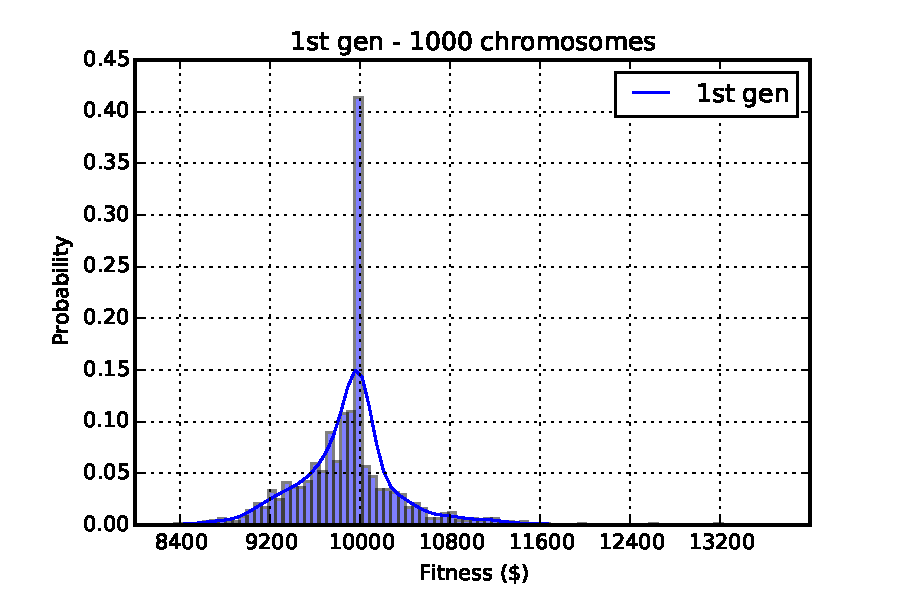
\includegraphics[width=0.9\columnwidth]{images/01r_1000.pdf}
	\end{figure}
\end{frame}

\begin{frame}{Results -- Selection}
	\begin{figure}[h]
	\centering
	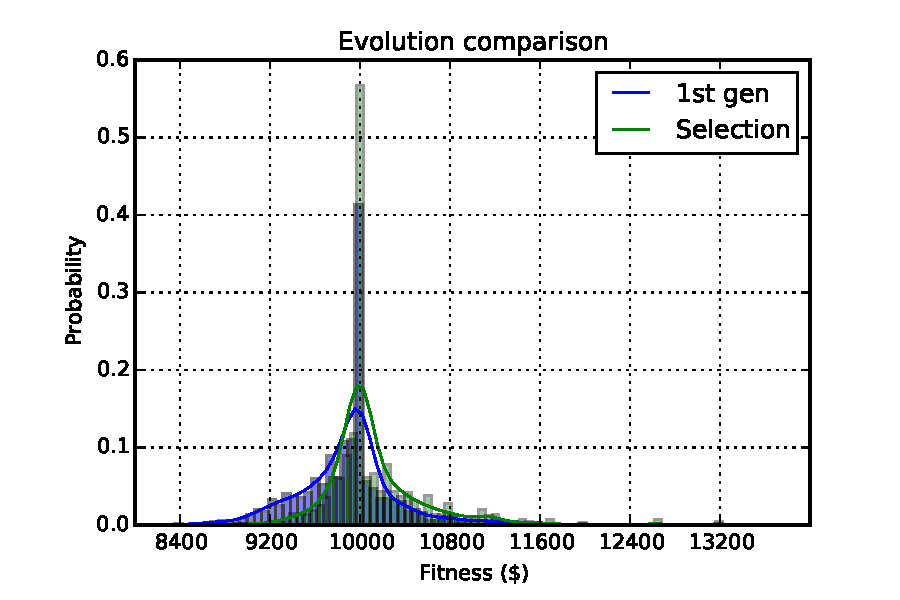
\includegraphics[width=0.9\columnwidth]{images/01r_1000_sel.pdf}
	\end{figure}
\end{frame}

%%%%%%%%%%%%
\subsection{100 chromosomes}
\begin{frame}{Results -- First generation 100 chromosomes}
	\begin{figure}[h]
	\centering
	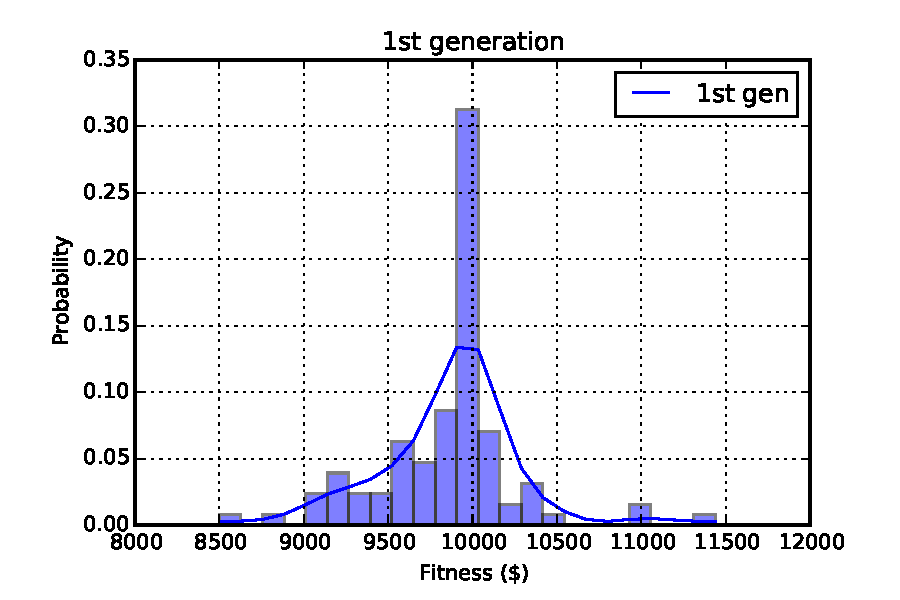
\includegraphics[width=0.9\columnwidth]{images/01r_100.pdf}
	\end{figure}
\end{frame}

\begin{frame}{Results -- Selection}
	\begin{figure}[h]
	\centering
	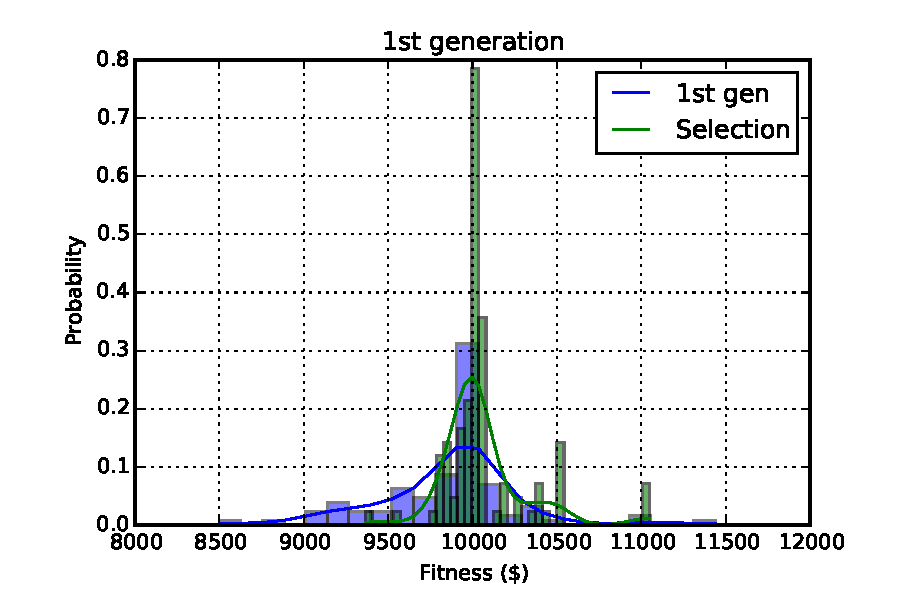
\includegraphics[width=0.9\columnwidth]{images/01r_100_sel1.pdf}
	\end{figure}
\end{frame}

\begin{frame}{Results -- Selection, crossover and mutation}
	\begin{figure}[h]
	\centering
	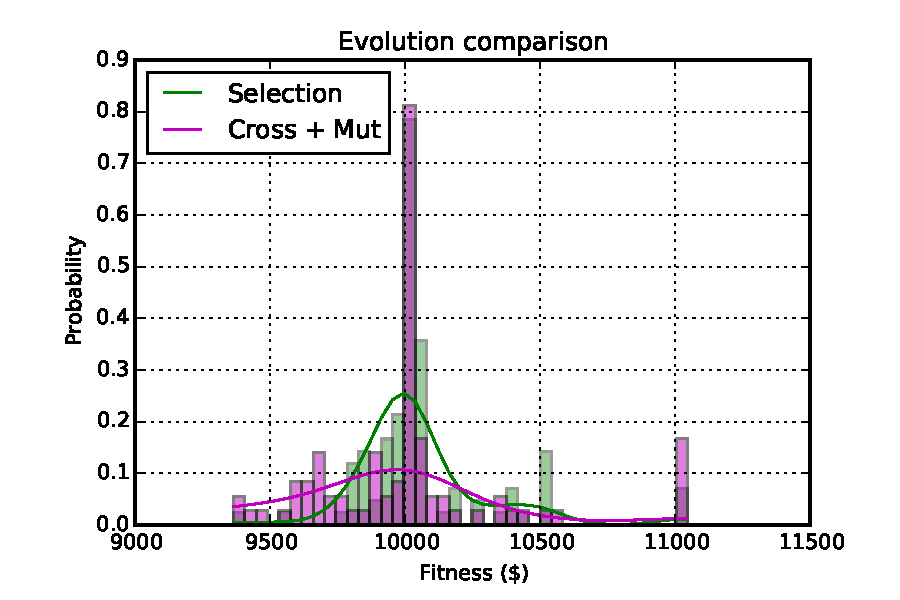
\includegraphics[width=0.9\columnwidth]{images/sel_x_cross_mut.pdf}
	\end{figure}
\end{frame}

\begin{frame}{Results -- Crossover, mutation and selection}
	\begin{figure}[h]
	\centering
	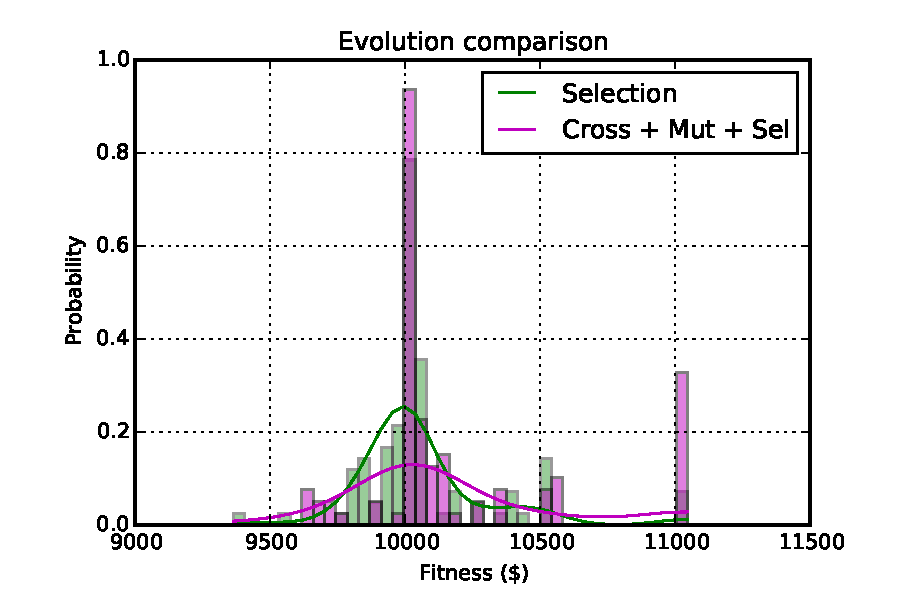
\includegraphics[width=0.9\columnwidth]{images/01r_100_cr_mut_sel.pdf}
	\end{figure}
\end{frame}

\begin{frame}{Results -- 10th generation}
	\begin{figure}[h]
	\centering
	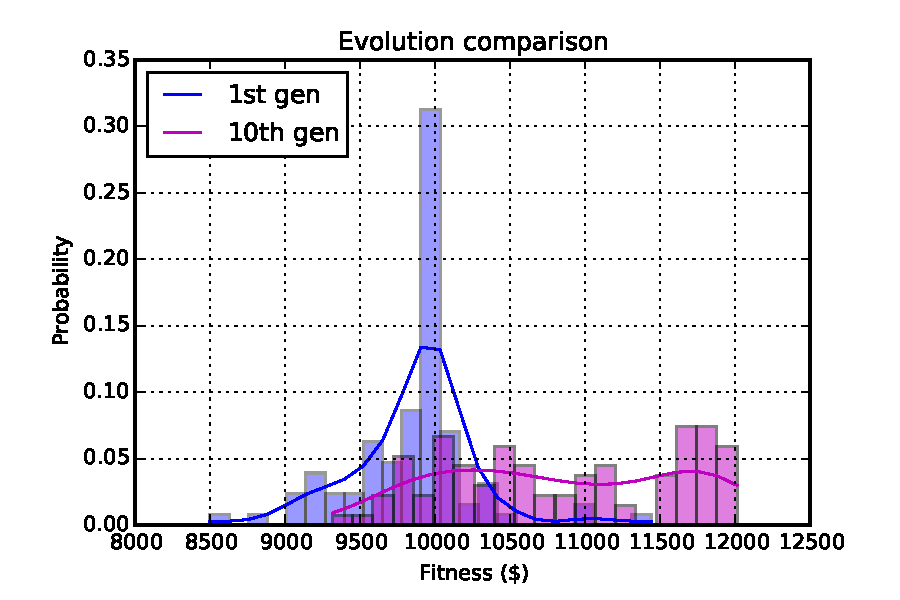
\includegraphics[width=0.9\columnwidth]{images/10r_100.pdf}
	\end{figure}
\end{frame}

\begin{frame}{Results -- 20th generation}
	\begin{figure}[h]
	\centering
	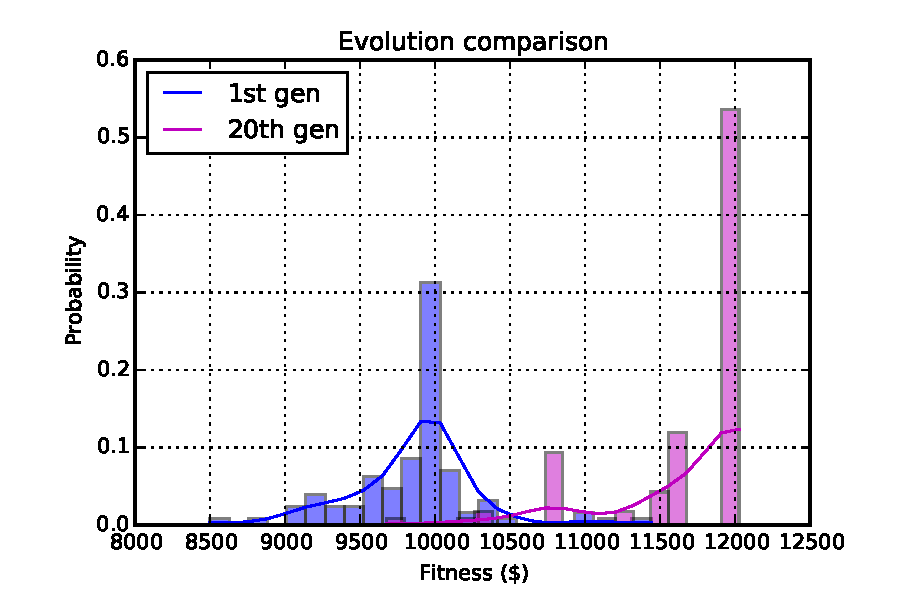
\includegraphics[width=0.9\columnwidth]{images/20r_100.pdf}
	\end{figure}
\end{frame}

\begin{frame}{Results -- 30th generation}
	\begin{figure}[h]
	\centering
	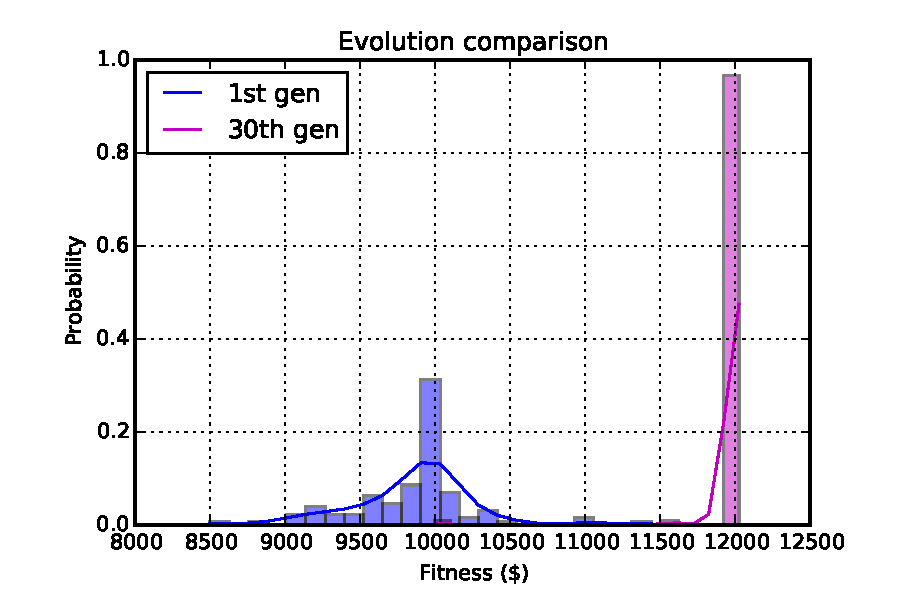
\includegraphics[width=0.9\columnwidth]{images/30r_100.pdf}
	\end{figure}
\end{frame}


%%%%%%%%%%%%
\subsection{100 chromosomes with seed}
\begin{frame}{Results -- First generation 100 chromosomes around seed}
	\begin{figure}[h]
	\centering
	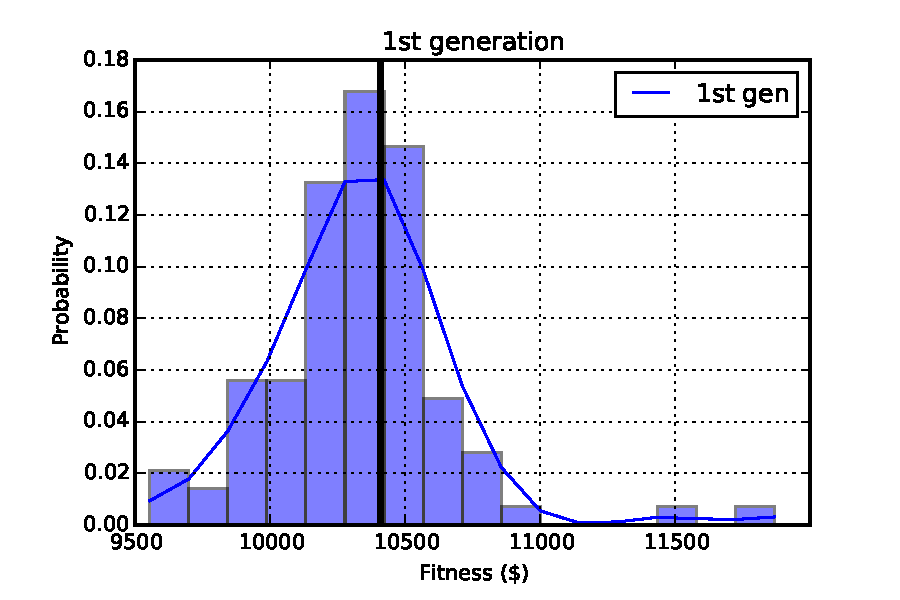
\includegraphics[width=0.9\columnwidth]{images/01l_100.pdf}
	\end{figure}
\end{frame}

\begin{frame}{Results -- Selection}
	\begin{figure}[h]
	\centering
	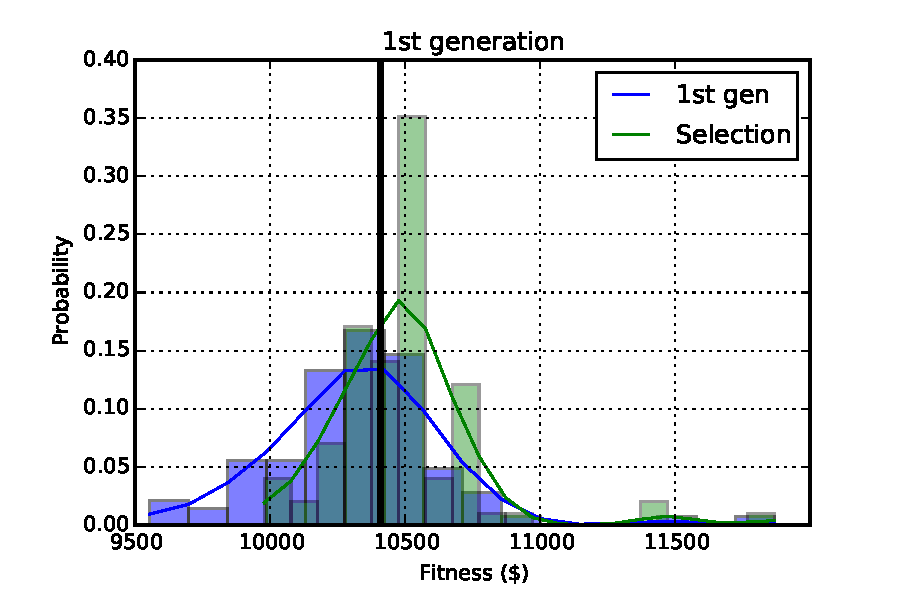
\includegraphics[width=0.9\columnwidth]{images/01l_100_sel1.pdf}
	\end{figure}
\end{frame}

\begin{frame}{Results -- Selection, crossover and mutation}
	\begin{figure}[h]
	\centering
	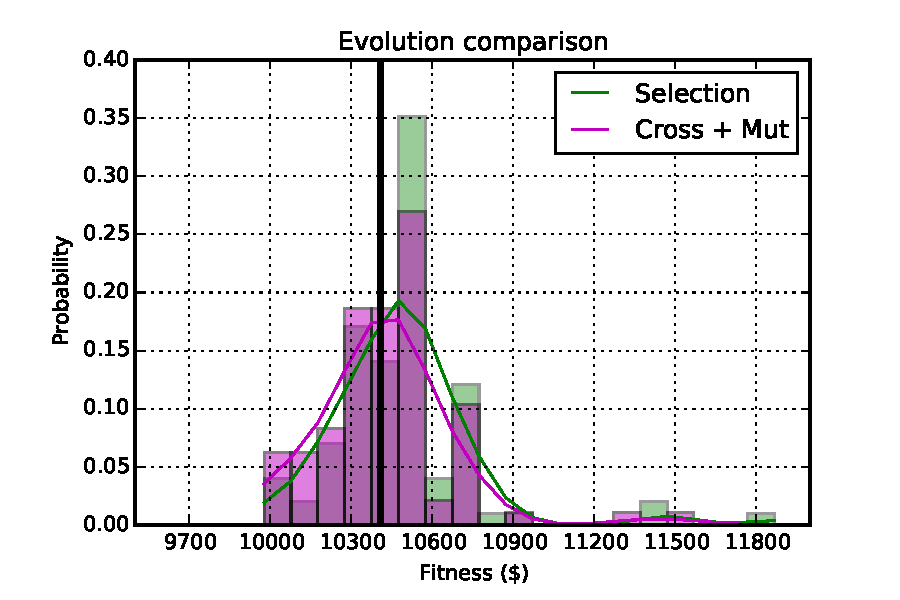
\includegraphics[width=0.9\columnwidth]{images/01l_100_cr_mut.pdf}
	\end{figure}
\end{frame}

\begin{frame}{Results -- Crossover, mutation and selection}
	\begin{figure}[h]
	\centering
	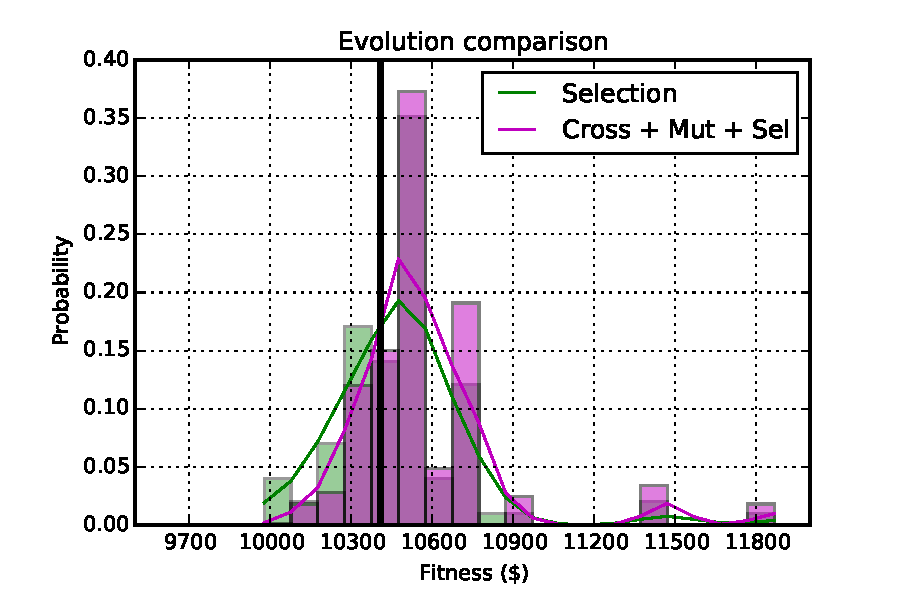
\includegraphics[width=0.9\columnwidth]{images/01l_100_cr_mut_sel.pdf}
	\end{figure}
\end{frame}

\begin{frame}{Results -- 10th generation}
	\begin{figure}[h]
	\centering
	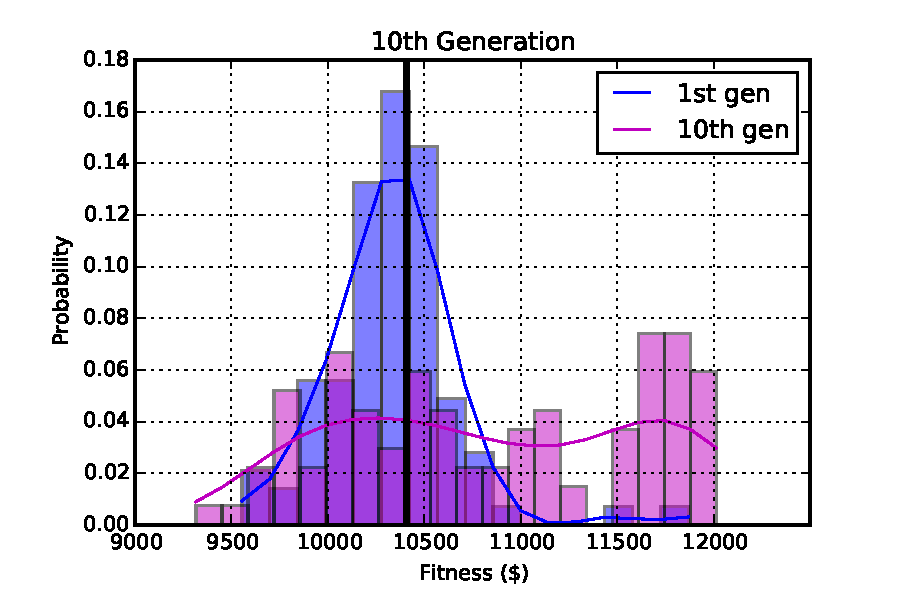
\includegraphics[width=0.9\columnwidth]{images/10l_100.pdf}
	\end{figure}
\end{frame}

\begin{frame}{Results -- 20th generation}
	\begin{figure}[h]
	\centering
	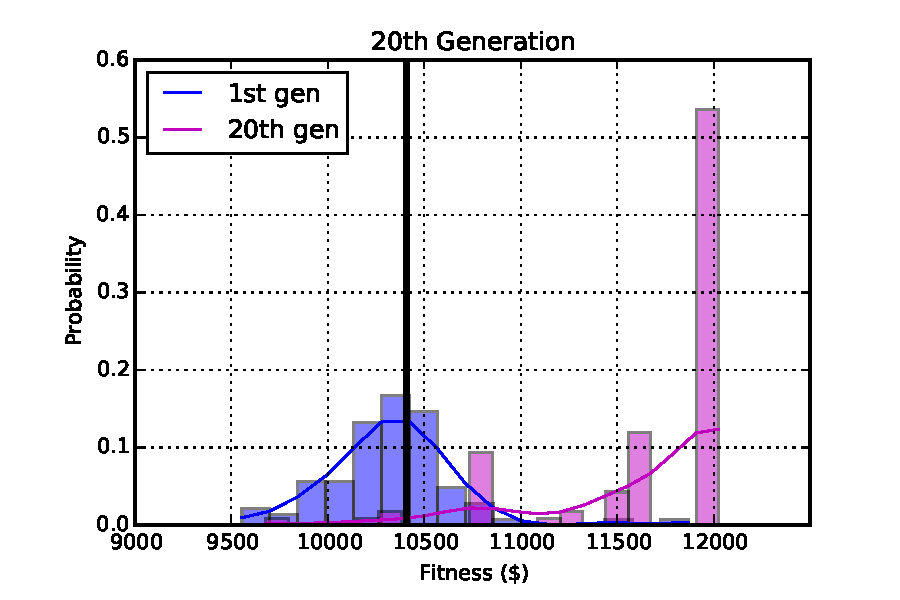
\includegraphics[width=0.9\columnwidth]{images/20l_100.pdf}
	\end{figure}
\end{frame}

\begin{frame}{Results -- 30th generation}
	\begin{figure}[h]
	\centering
	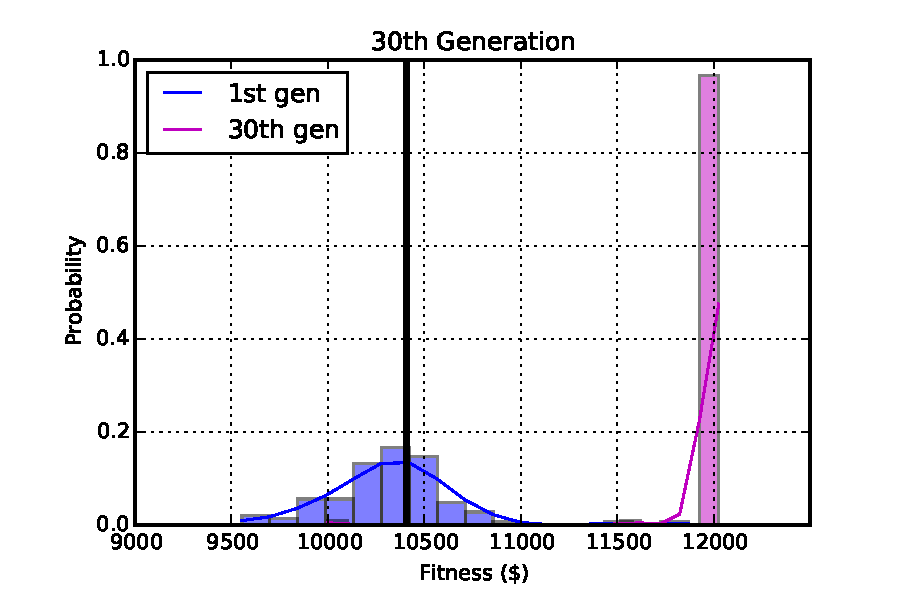
\includegraphics[width=0.9\columnwidth]{images/30l_100.pdf}
	\end{figure}
\end{frame}
%
%
%
%
%
%
%
%
%
%
%
%
%
%
% sections in the presentation
\begin{comment}
\section{Primeira}
\subsection{Algoritmo}
\begin{frame}{Algoritmo genético -- SSC5858}
\begin{center}
\scalebox{0.65}{
\begin{minipage}{1.3\linewidth}

\begin{algorithm}[H]
\caption{AG para criação de regras}
\begin{algorithmic}[1]
	\State $args[] = [size, crossover, mutation, elitism, imigration, tournamentSize, port]$
	\State let $population$ be a new \textsc{Population}($args$)
	\For{$i = 1$ to $maxGenerations$}
		\State Evaluate population
		\State Plot current evolution
		\If{didn't improve for $maxNotImproved$}
			\State break
		\EndIf
		\State Evolve population to the next generation
	\EndFor
\end{algorithmic}
\end{algorithm}
\end{minipage}%
}
\end{center}
\end{frame}

\begin{frame}{Algoritmo genético -- SSC5858}
\begin{center}
\scalebox{0.65}{
\begin{minipage}{1.3\linewidth}

\begin{algorithm}[H]
\caption{Evolução da população}
\begin{algorithmic}[1]
\Procedure{evolve}{}
	\State Select $elitism*size$ chromosomes to be in the next generation
	\If{$(best-worst)/worst <= 0.08$}
		\State $imigration = 0.5$
	\EndIf
	\State Create $imigration*size$ chromosomes to be in the next generation
	\While{size of the next generation $< size$}
		\State $parent1 = $ best of random tournament selection with size $tournamentSize$
		\State $parent2 = $ best of random tournament selection with size $tournamentSize$
		\If{$crossover$ is applied}
			\State $childs = crossover(parent1, parent2)$
		\Else
			\State $childs = [parent1, parent2]$
		\EndIf
		\For{$child$ in $childs$}
			\If{$mutation$ is applied}
				\State $child = mutate(child)$
			\EndIf
		\EndFor
		\State Add childs to the next generation
		\State Order and trim the next generation by fitness
	\EndWhile
\EndProcedure
\end{algorithmic}
\end{algorithm}
\end{minipage}%
}
\end{center}
\end{frame}

\subsection{Cálculo do fitness}
\begin{frame}{Cálculo do \textit{fitness}}
	Avaliação da população é realizada em um \textit{backtest} com a ferramenta \textit{Systematic Investor Toolkit} em R.
	\begin{itemize}
		\item Servidor R carrega a ferramenta, os dados e fica escutando em uma porta
		\pause
		\item Cliente Python decodifica cromossomo e envia para o R
		\pause
		\item Servidor R realiza o \textit{backtest} e retorna o índice Sharpe da estratégia
\begin{equation*}
	\setlength\arraycolsep{2.5pt}
	\begin{array}{r c c c l}
		S_{a} & = & \frac{E[R_{a} - R_{b}]}{\sigma_a} & = & \frac{E[R_{a} - R_{b}]}{\sqrt{var[R_a-R_b]}}
	\end{array}
\end{equation*}
		\pause
		\item Cliente Python recebe o \textit{fitness} e segue para o próximo cromossomo
	\end{itemize}
\end{frame}

\subsection{Encodificação}
\begin{frame}{Encodificação}
\begin{figure}[H]
\centering
\includegraphics[width=\textwidth]{images/03.pdf}
\end{figure}
\end{frame}

\begin{frame}{Encodificação}
\begin{figure}[H]
\centering
\includegraphics[width=\textwidth]{images/02.pdf}
\end{figure}
\end{frame}

\begin{frame}{Encodificação}
\begin{figure}[H]
\centering
\includegraphics[width=\textwidth]{images/01_2.pdf}
\end{figure}
\end{frame}

\begin{frame}{Encodificação}
\begin{figure}[H]
\centering
\includegraphics[width=\textwidth]{images/01.pdf}
\end{figure}
\end{frame}

\subsection{Operadores}
\subsubsection{Cruzamento}
\begin{frame}{Operadores -- Cruzamento}
Chances iguais para cada tipo de operação
\begin{itemize}
		\pause
	\item 1 ponto -- Escolhe um ponto de corte e combina a parte 1 do primeiro cromossomo com a parte 2 do segundo
		\pause
	\item 2 pontos -- Escolhe dois pontos de corte e troca os setores do meio
		\pause
	\item Combinação
	\begin{itemize}
		\item Combinação linear $\alpha c_1 + (1-\alpha)c_2, \alpha \in [0,1)$, caso $c$ seja numérico
		\item Escolhe entre os dois cromossomos, caso $c$ não seja numérico
	\end{itemize}
\end{itemize}
\end{frame}

\subsubsection{Mutação}
\begin{frame}{Operadores -- Mutação}
Chances iguais para cada tipo de operação
\begin{itemize}
		\pause
	\item Gera nova regra aleatória
		\pause
	\item Gera novos parâmetros
		\pause
	\begin{itemize}
		\item Alterna operador lógico
		\item Alterna operador relacional
		\item Gera novo indicador técnico aleatório
		\item Gera novos parâmetros numéricos aleatórios
	\end{itemize}
\end{itemize}
\end{frame}

\end{comment}
\section{References}
\begin{frame}[allowframebreaks]{References}
	\begingroup
	\footnotesize
	\bibliographystyle{plainnat}
	\bibliography{bibliography}
	\endgroup
\end{frame}

\end{document}
